\documentclass[12pt, twoside]{article}
\usepackage{jmlda}
\usepackage{url}
\usepackage{graphicx}
\newcommand{\hdir}{.}

\begin{document}

\title
    {Классификация траекторий физических систем с помощью лагранжевых нейронных сетей}
\author
    {А.\,И.~Богданов, С.\,К.~Панченко, В.\,В.~Стрижов} 
\email
    {bogdanov.ai@phystech.edu; panchenko.sk@phystech.edu; strijov@phystech.edu}
\abstract{
    В работе решается задача классификации траекторий физических систем. Квазипериодическая динамика системы аппроксимируется лагранжианом, который восстанавливается по обобщённым координатам с помощью лагранжевой нейронной сети. Показано, что для параметров таких сетей выполняется гипотеза компактности: векторы параметров, соответствующие траекториям различных классов, оказываются разделимы в своём пространстве. Проводится эксперимент на датасете PAMAP2, результаты которого подтверждают, что параметры лагранжевых нейронных сетей действительно являются информативным признаковым описанием для задачи классификации. 

\bigskip

\noindent
\textbf{Ключевые слова}: \emph {физическая система, лагранжиан, лагранжева нейронная сеть}

}

\maketitle

\section{Введение}
 
    Для моделирования динамики физических систем часто используется лагранжева динамика \cite{landau1976mechanics}. В соответствии с ней выбирается набор обобщенных координат, который полностью описывает физическую систему, затем строится лагранжиан $L$, который определяется как разница между кинетической энергией ($T$) и потенциальной энергией ($V$) системы

    $$L = T - V.$$
    Для получения уравнений движения нужно воспользоваться уравнением Эйлера-Лагранжа

    $$\frac{d}{dt} \frac{\partial L}{\partial \dot{\mathbf{q}}} - \frac{\partial L}{\partial \mathbf{q}} = 0,$$
    полученным из принципа наименьшего действия.

    Нейронные сети упрощают моделирование динамики физических систем и классификацию ее траекторий. Для их использования не требуются знание лагранжиана и решение сложных систем дифференциальных уравнений. 
    
    Лагранжева нейронная сеть (LNN) \cite{cranmer2020lagrangian} аппроксимирует лагранжиан системы, который позволяет перейти к более простому математическому представлению физической системы. С помощью уравнения Эйлера-Лагранжа из этого лагранжиана можно восстановить динамику этой физической системы.

    Для параметров лагранжевых нейронных сетей выдвигается гипотеза компактности: векторы параметров, соответствующие траекториям различных классов, оказываются разделимы в своём пространстве. Эти параметры являются признаками в задаче классификации траекторий системы.
    
    Для проверки поставленной гипотезы проводится вычислительный эксперимент на датасете PAMAP2 \cite{PAMAP2}, который содержит размеченные траектории движений человека во время различных активностей.

\newpage
    
\section{Постановка задачи классификации траекторий физических систем}

Задана выборка с метками из $n$ траекторий

    $$\{ \mathcal{D}_j, z_j\}_{j=1}^n,$$ 
    где:
    \begin{itemize}

        \item[$\bullet$] $\mathcal{D}_j = \{ \mathbf{x}_i^{(j)}, \mathbf{y}_i^{(j)} \}_{i=1}^{m_j}$ ~-- $j$-ая траектория,

        \item[$\bullet$] $\mathbf{x}_i^{(j)} = (\mathbf{q}_i^{(j)}, \mathbf{\dot{q}}_i^{(j)})$ ~-- координаты $j$-ой траектории движения физической системы, 

        \item[$\bullet$] $\mathbf{y}_i^{(j)} = \mathbf{\dot{x}}_i^{(j)} = (\mathbf{\dot{q}}_i^{(j)}, \mathbf{\ddot{q}}_i^{(j)})$ ~-- динамика движения физической системы на $j$-ой траектории, 

        \item[$\bullet$] $\mathbf{q}_i^{(j)} \in \mathbb{R}^r$ ~-- вектор обобщенных координат,

        \item[$\bullet$] $r$ ~-- количество координат,

        \item[$\bullet$] $m_j$ ~-- длина $j$-ой траектории,

        \item[$\bullet$] $z_j$ ~-- метка $j$-ой траектории.
        
    \end{itemize}
        
    \paragraph{Задачи регрессии восстановления лагранжиана}

        Сведём задачу моделирования лагранжиана системы к задаче регрессии. Регрессионная модель для траектории $D_j$ выбирается из класса нейронных сетей

        $$\mathbf{f_j} \colon (\mathbf{x}, \mathbf{w}) \to \mathbf{y}, \quad \mathbf{x} \in \mathbb{R}^{2 \times r}, \quad \mathbf{y} \in \mathbb{R}^{2 \times r},$$ 
        где: 
    
        \begin{itemize}
    
            \item[$\bullet$] $\mathbf{w} \in \mathbb{W}$ ~-- параметры модели, 

            \item[$\bullet$] $\hat{\mathbf{y}}_i^{(j)} = \mathbf{f}_j (\mathbf{x}_i^{(j)}, \mathbf{w}) \in \mathbb{R}^{2 \times r}$ ~-- предсказанная динамика движения физической системы на $j$-ой траектории,
        
            \item[$\bullet$] $\mathbf{X}_j = \bigcup_{i=1}^{m_j} \mathbf{x}_i^{(j)}$ ~-- матрица координат $j$-ой траектории движения физической системы,
            
            \item[$\bullet$] $\mathbf{Y}_j = \bigcup_{i=1}^{m_j} \mathbf{y}_i^{(j)}$ ~-- матрица динамики $j$-ой траектории движения физической системы,
            
            \item[$\bullet$] $\hat{\mathbf{Y}}_j = \bigcup_{i=1}^{m_j} \hat{\mathbf{y}}_i^{(j)}$ ~-- предсказанная матрица динамики $j$-ой траектории движения физической системы.
        
        \end{itemize}

        Задача моделирования динамики системы представлена в виде задачи минимизации квадратичной ошибки

        $$\mathcal{L}(\textbf{w}) = \mathcal{L}(\mathbf{w} | \mathbf{X}_j, \mathbf{Y}_j) = \| \hat{\mathbf{Y}}_j - \mathbf{Y}_j \|_2^2,$$
    
        $$\textbf{w}_j^* = \argmin_{\mathbf{w} \in \mathbb{W}} \left( \mathcal{L}(\textbf{w}) \right).$$

    \paragraph{Задачи классификации траекторий по лагранжианам}

        После решения задачи моделирования лагранжиана получаем задачу классификации

        $$\{\textbf{w}^*_j, z_j\}_{j=1}^n,$$
        где $\textbf{w}^*_j$ ~-- коэффициенты аппроксимированного лагранжиана $j$-ой траектории.
    
        Для ее решения используются различные методы классификации, среди которых: логистическая регрессия, ядерный метод с гауссовским ядром, случайный лес.

\section{Лагранжевы нейронные сети}

    \paragraph{Лагранжева динамика}		

        Лагранжев формализм \cite{cranmer2020lagrangian} моделирует физическую систему с координатами траектории $\mathbf{x_t} = (\mathbf{q}, \dot{\mathbf{q}})$, которая начинается в состоянии $\mathbf{x}_0$ и заканчивается в состоянии $\mathbf{x}_1$. Определяется функционал, называющийся действием

        $$S=\int\limits_{t_0}^{t_1} L dt,$$
        показывающий путь, по которому координаты $\mathbf{x}_t$ пройдут из $\mathbf{x}_0$ в $\mathbf{x}_1$ в промежуток времени от $t_0$ до $t_1$. Путь минимизирует действие $S$, что приводит к уравнению Эйлера-Лагранжа, определяющему динамику системы

        $$\frac{d}{dt} \frac{\partial L}{\partial \dot{\mathbf{q}}} = \frac{\partial L}{\partial \mathbf{q}}$$

        Ускорение каждой компоненты системы $ \ddot{\mathbf{q}}$ может быть напрямую получено из данного уравнения

        $$\begin{aligned}
            \frac{\partial}{\partial \dot{\mathbf{q}}} \frac{dL}{dt} &= \frac{\partial L}{\partial \mathbf{q}}\\
            \frac{\partial}{\partial \dot{\mathbf{q}}} \left( \frac{\partial L}{\partial \mathbf{q}} \frac{dq}{dt} + \frac{\partial L}{\partial \dot{\mathbf{q}}} \frac{d\dot{\mathbf{q}}}{dt} \right) &= \frac{\partial L}{\partial \mathbf{q}} \\
            \frac{\partial}{\partial \dot{\mathbf{q}}} \left( \frac{\partial L}{\partial \mathbf{q}} \dot{\mathbf{q}} + \frac{\partial L}{\partial \dot{\mathbf{q}}} \ddot{\mathbf{q}} \right) &= \frac{\partial L}{\partial \mathbf{q}} \\ 
            \frac{\partial}{\partial \dot{\mathbf{q}}} \frac{\partial L}{\partial \mathbf{q}} \dot{\mathbf{q}} + \frac{\partial}{\partial \dot{\mathbf{q}}} \frac{\partial L}{\partial \dot{\mathbf{q}}} \ddot{\mathbf{q}} &= \frac{\partial L}{\partial \mathbf{q}} \\
            \frac{\partial}{\partial \dot{\mathbf{q}}} \frac{\partial L}{\partial \dot{\mathbf{q}}} \ddot{\mathbf{q}} &= \frac{\partial L}{\partial \mathbf{q}} - \frac{\partial}{\partial \dot{\mathbf{q}}} \frac{\partial L}{\partial \mathbf{q}} \dot{\mathbf{q}} \\
            \ddot{\mathbf{q}} &= \left( \frac{\partial}{\partial \dot{\mathbf{q}}} \frac{\partial L}{\partial \dot{\mathbf{q}}} \right)^{-1} \left[ \frac{\partial L}{\partial \mathbf{q}} - \frac{\partial}{\partial \dot{\mathbf{q}}} \frac{\partial L}{\partial \mathbf{q}} \dot{\mathbf{q}} \right] \\
            \ddot{\mathbf{q}} &= \left( \nabla_{\dot{\mathbf{q}}} \nabla_{\dot{\mathbf{q}}}^T L \right)^{-1} \left[ \nabla_{\mathbf{q}} L - \left( \nabla_{\dot{\mathbf{q}}} \nabla_{\mathbf{q}}^T L \right) \dot{\mathbf{q}} \right].
        \end{aligned}$$

    \paragraph{Лагранжева нейронная сеть}

        В работе \cite{cranmer2020lagrangian} предложено в нейронную сеть

        $$f: \mathbf{X} = (\mathbf{q}, \mathbf{\dot{q}}) \rightarrow \mathbf{Y}$$
        добавить априорные знания о физике системы, учитывая лагранжиан системы
    
        $$f: \mathbf{X} = (\mathbf{q}, \mathbf{\dot{q}}) \rightarrow L.$$

        Ключевой идеей является параметризовать нейронной сетью лагранжиан $L$, получить выражение ограничения Эйлера-Лагранжа и обратно распространить ошибку через полученные ограничения
    
        $$\ddot{\mathbf{q}} = \left( \nabla_{\dot{\mathbf{q}}} \nabla_{\dot{\mathbf{q}}}^T L \right)^{-1} \left[ \nabla_{\mathbf{q}} L - \left( \nabla_{\dot{\mathbf{q}}} \nabla_{\mathbf{q}}^T L \right) \dot{\mathbf{q}} \right].$$

        На рисунке \ref{fig: LNN} представлена схема работы LNN для задачи моделирования динамики системы. В качестве нейронной сети $f: \mathbf{X} = (\mathbf{q}, \mathbf{\dot{q}}) \rightarrow L$ берется полносвязная сеть с 3-мя слоями.

        \begin{figure}[H]
            \centering
            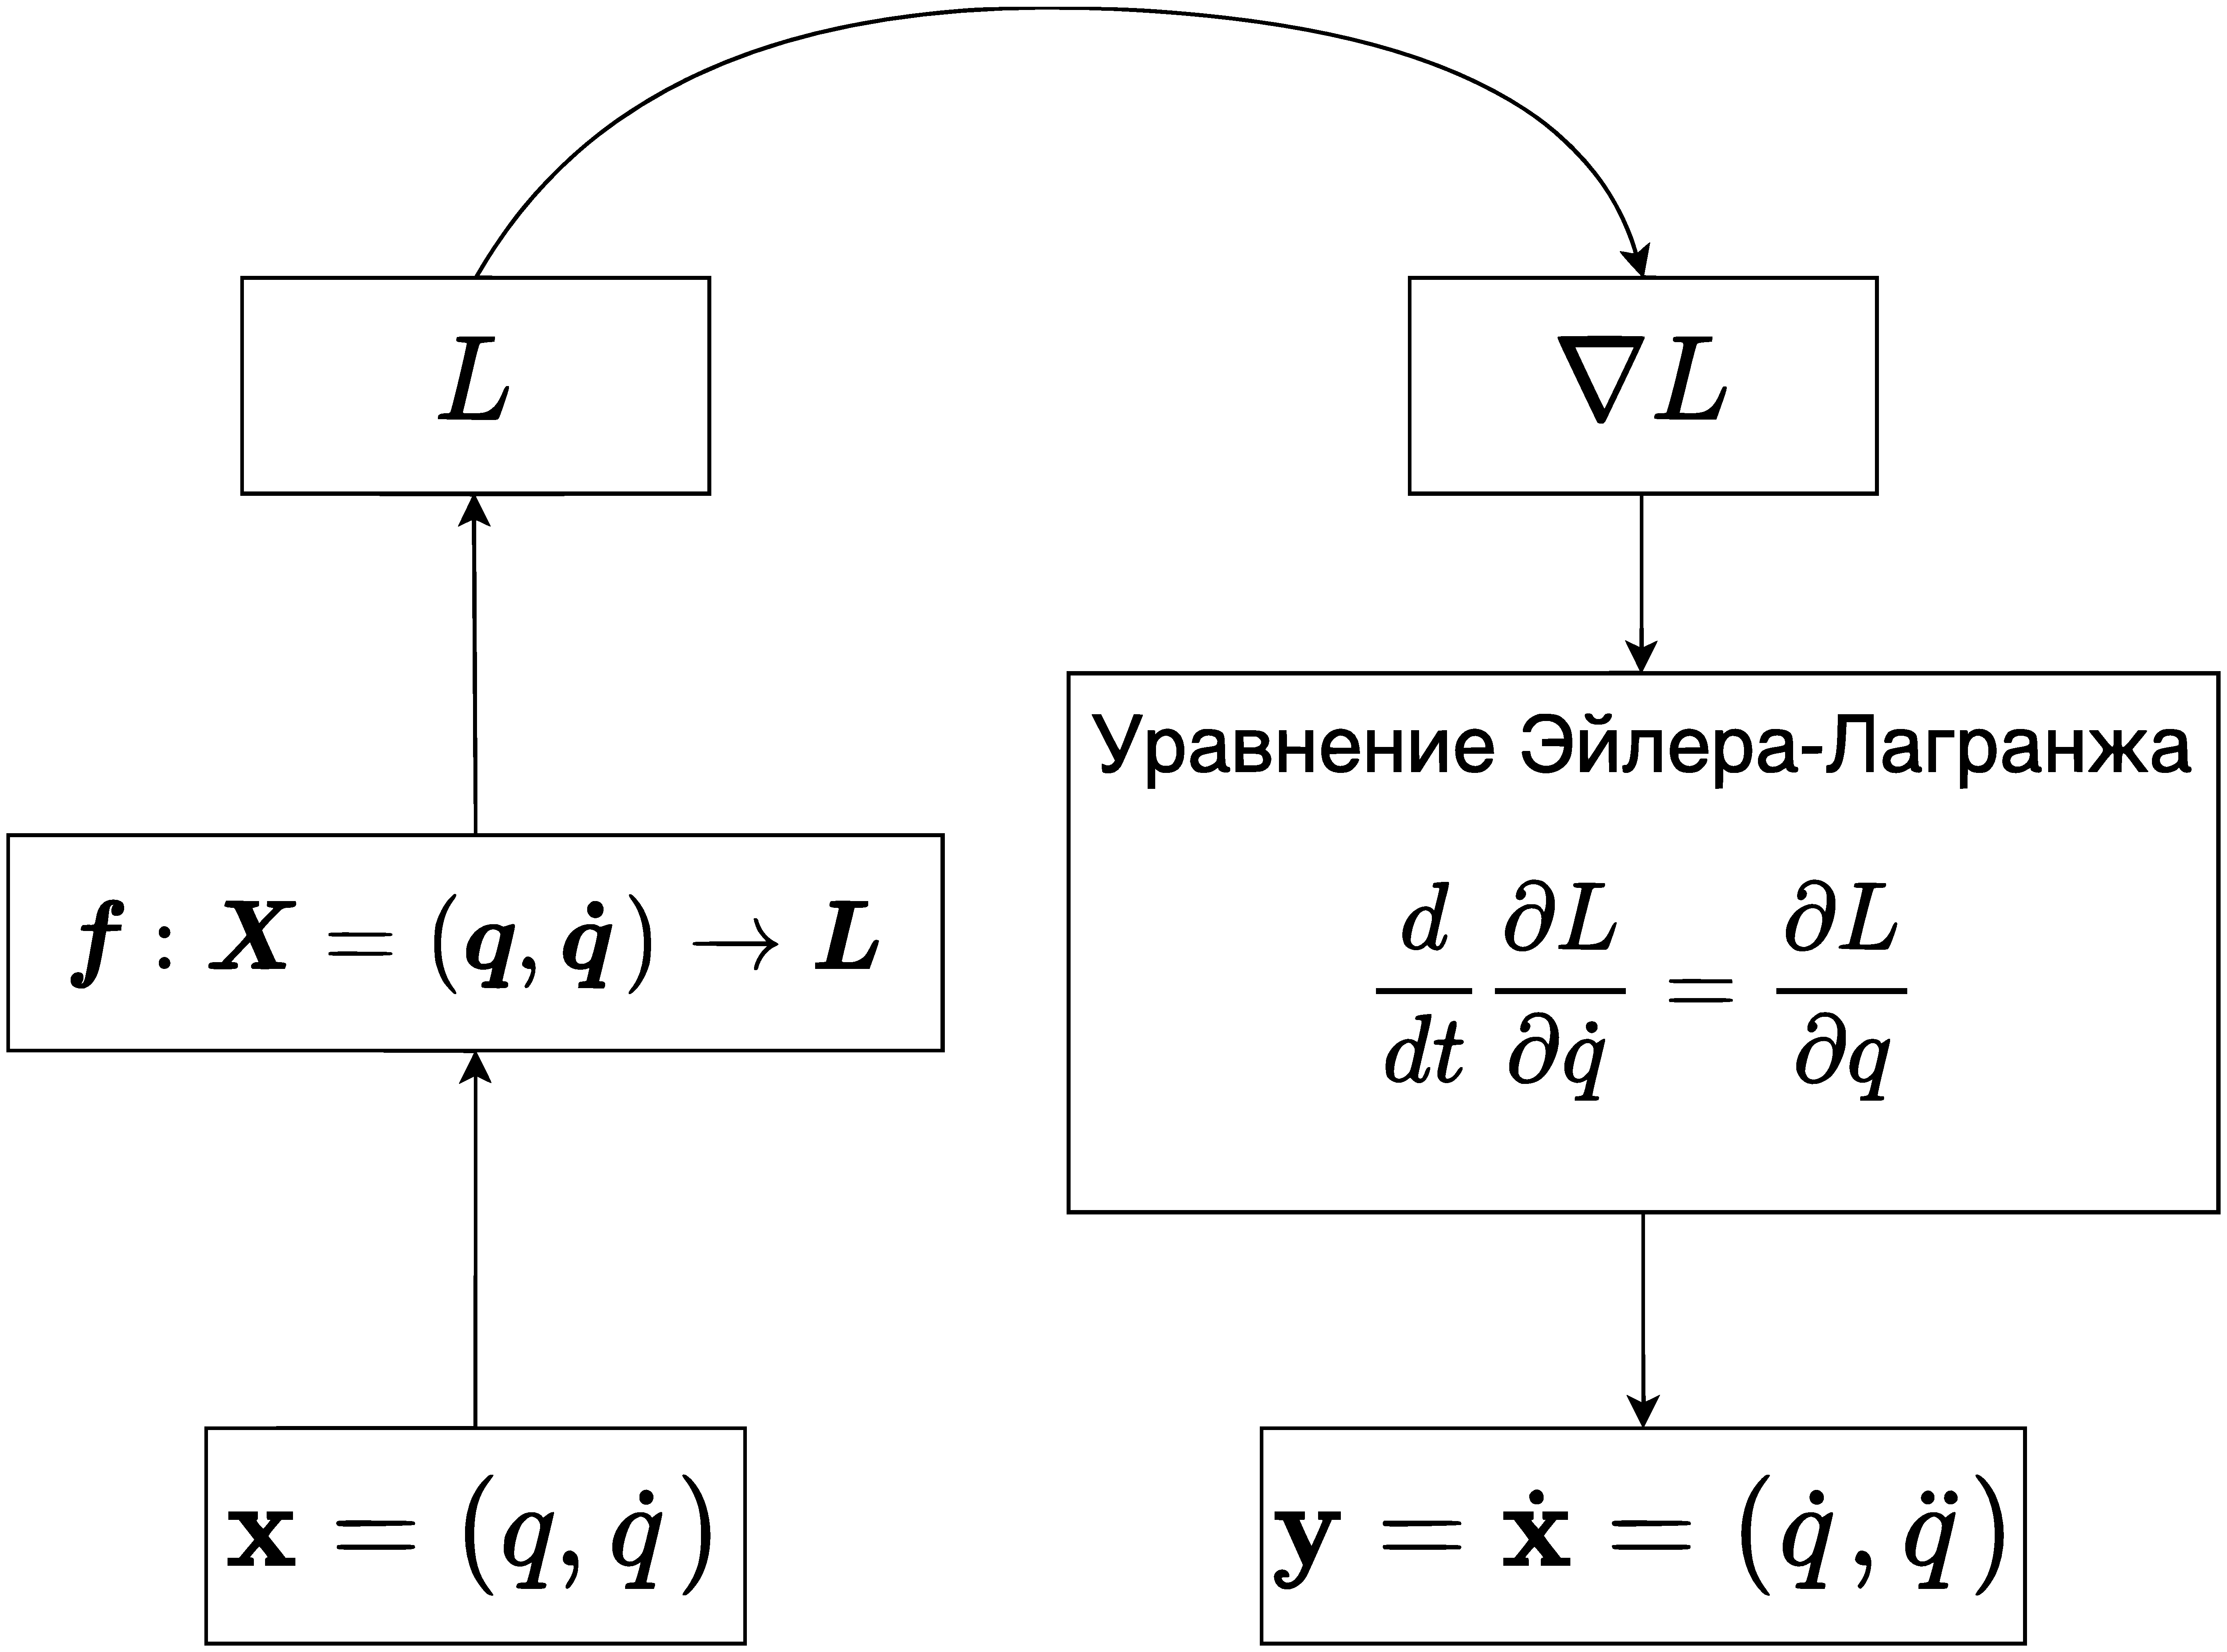
\includegraphics[width=0.7\textwidth]{LNN.eps}
            \caption{Схема работы LNN для задачи моделирования динамики физической системы.}
            \label{fig: LNN}
        \end{figure}
    
\section{Вычислительный эксперимент}

    Для эксперимента используется датасет PAMAP2 \cite{PAMAP2}.

    \paragraph{Данные}
    
        \begin{itemize}

            \item[$\bullet$] Количество акселерометров: 3,
                    
                    \begin{itemize}

                        \item[$\bullet$] На запястье рабочей руки,

                        \item[$\bullet$] На рабочей ноге,

                        \item[$\bullet$] На груди.

                    \end{itemize}

            \item[$\bullet$] Частота акселерометров: 100 Гц,
            
            \item[$\bullet$] Количество классов: K = 12,

            \item[$\bullet$] Количество испытуемых: 9 человек.

        \end{itemize}

    Для эксперимента использовались данные с рабочей ноги и 4 класса.

    \paragraph{Подготовка данных \cite{processing}}

        Данные подверглись следующей процедуре предобработки:
        
        \begin{itemize}
    
            \item[$\bullet$] Восстановлены пропуски данных, связанные с тем, что датчик может пропустить такт. Для использовалась сплайн-интерполяция.

            \item[$\bullet$] Посчитаны отсутствующие необходимые данные: ускорения и координаты. Для их получения использовались методы вычислительной математики.

                \begin{itemize}

                    \item[$\bullet$] Для получения ускорения используется аппроксимация 2-го порядка:
                         $$f'(x_i) \approx \frac{f(x_{i + 1}) - f(x_{i - 1})}{2h},$$

                    \item[$\bullet$] Для получения координаты используется метод Симпсона 3-го порядка аппроксимации:
                        $$\int\limits_a^b f(x) dx \approx \frac{h}{3} \sum\limits_{k = 1}^{N - 1} \left( f(x_{k + 1} + 4f(x_k) + f(x_{k - 1}) \right).$$

                \end{itemize}

        \end{itemize}

    \paragraph{Эксперимент \cite{experiment, master-tesis}}

        Фиксируется сбалансированная подвыборка из датасета PAMAP2. Для каждой траектории из этой подвыборки с помощью LNN моделируется лагранжиан. Параметры обученной нейронной сети представляют собой признаковое описание данной траектории. Затем с помощью различных классификаторов, таких как логистическая регрессия, ядерный метод с гауссовским ядром, случайный лес, определяется принадлежность к классу.
        
        Избыточная размерность нового признакового описания снижается с помощью метода главных компонент (PCA). Проекции признаков на 2D на и 3D приведены, соответственно, на рисунке \ref{fig: 2D} и \ref{fig: 3D}.

        \begin{figure}[H]
            \centering
            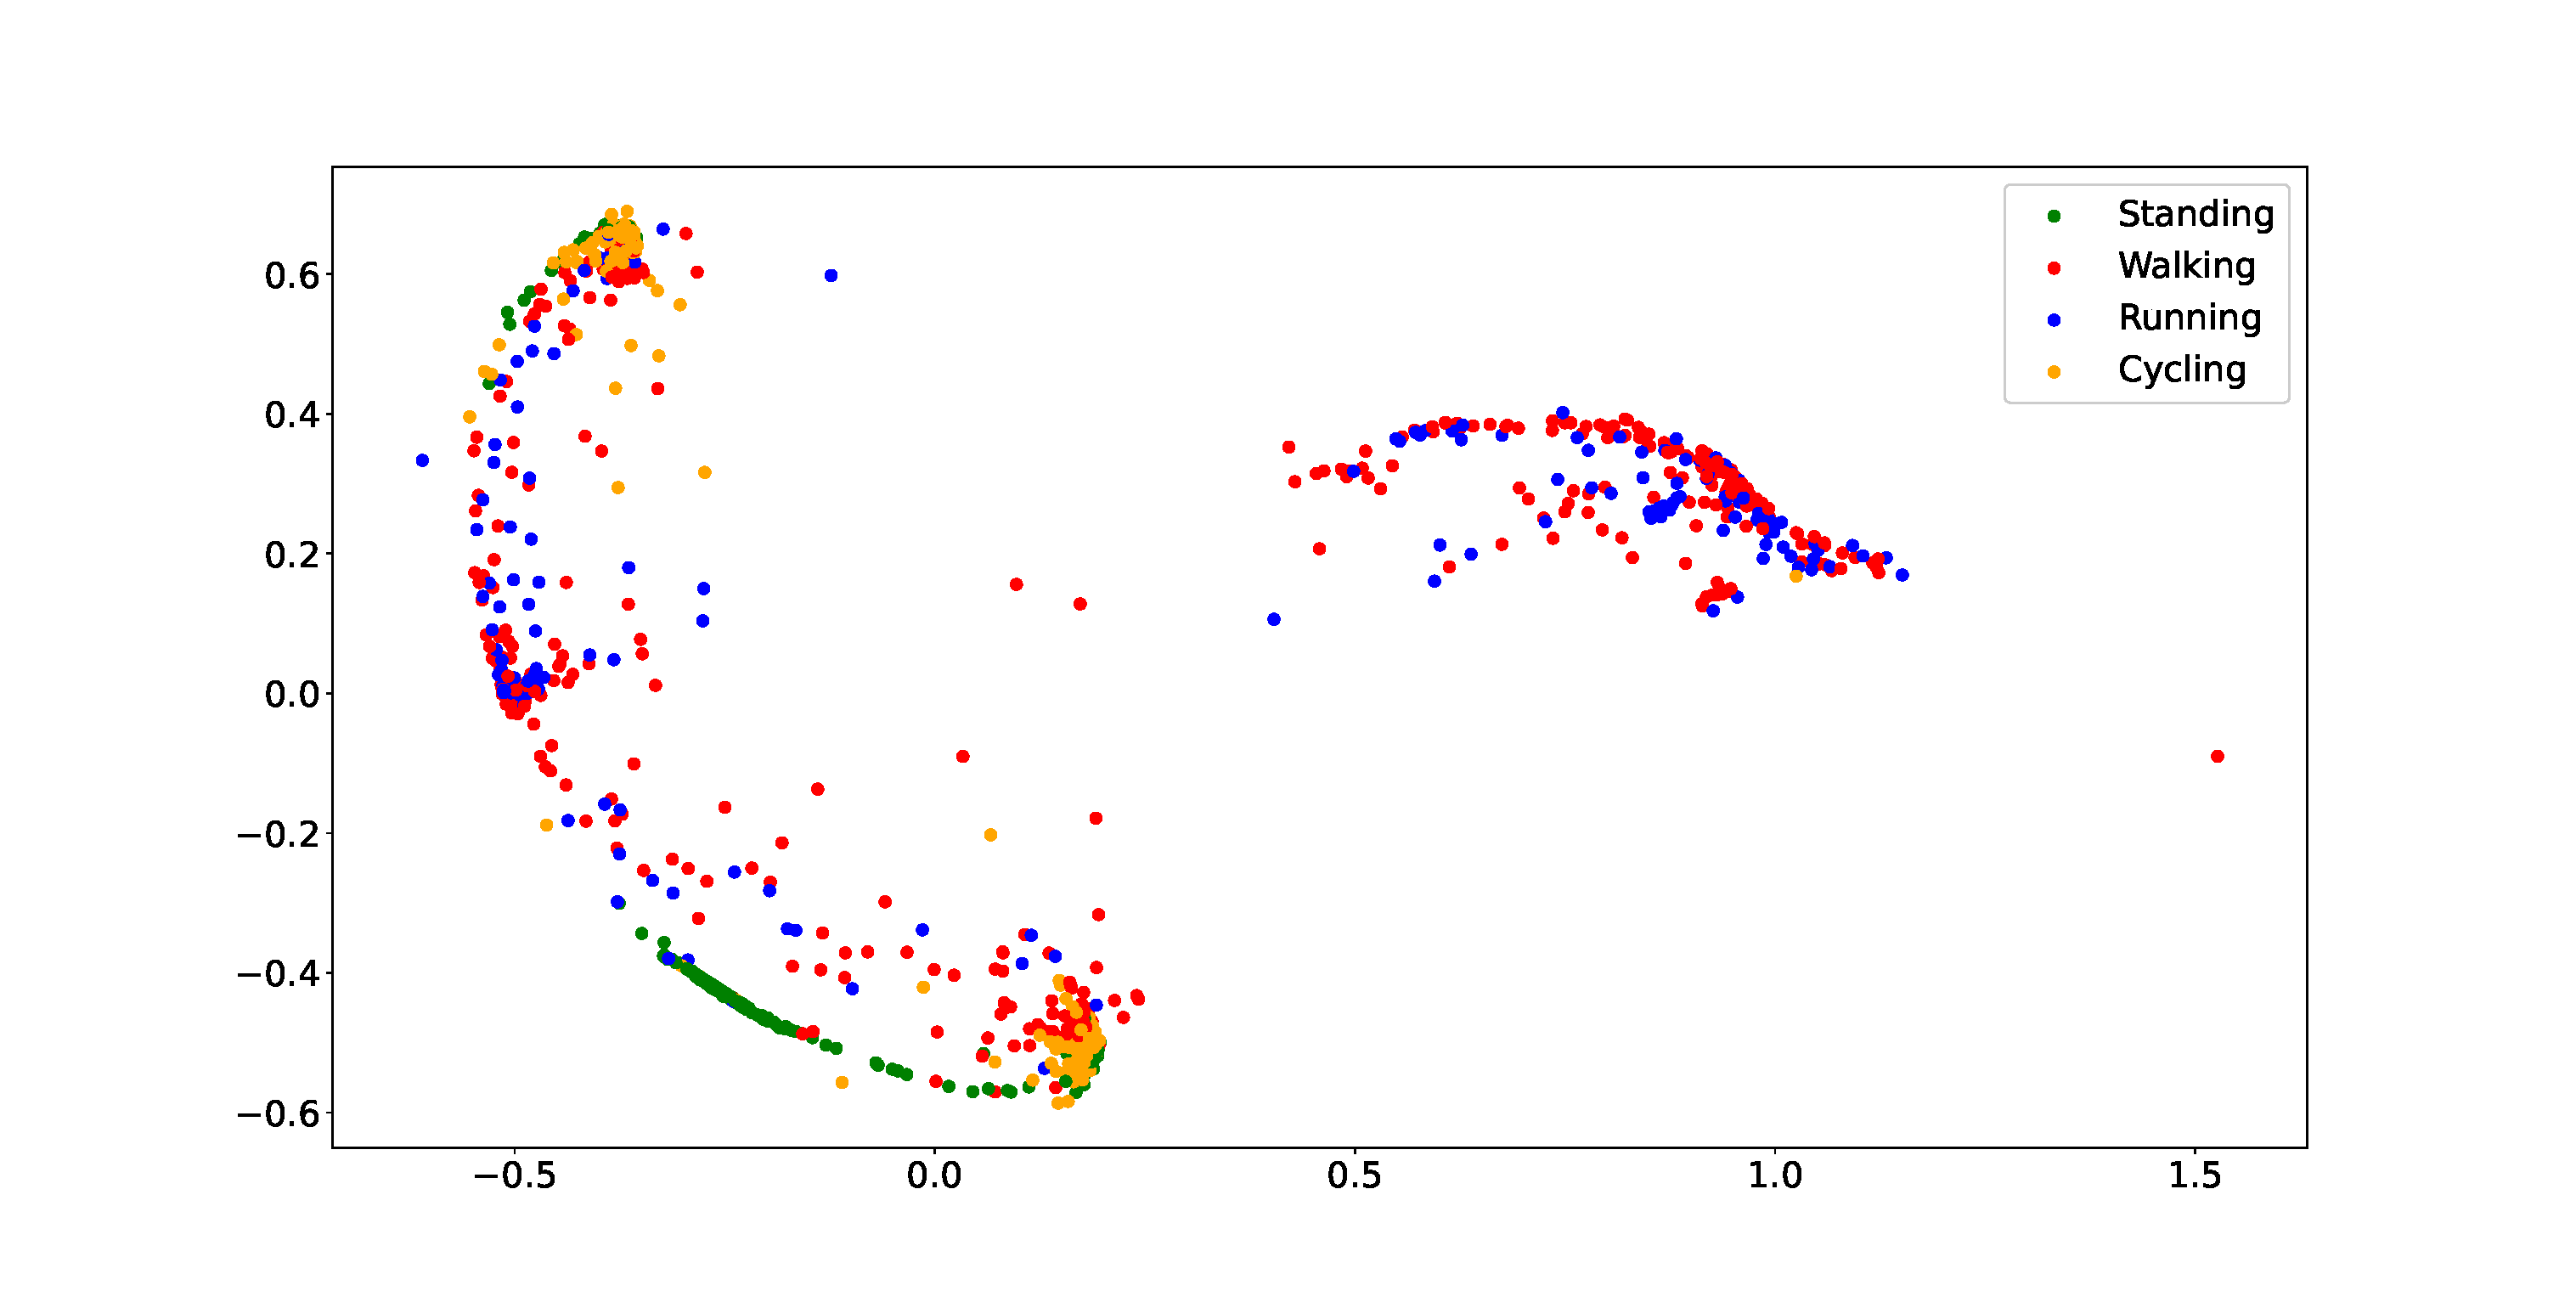
\includegraphics[width=0.7\textwidth]{Data_2D.eps}
            \caption{Распределения данных в 2D}
            \label{fig: 2D}
        \end{figure}

        \begin{figure}[H]
            \centering
            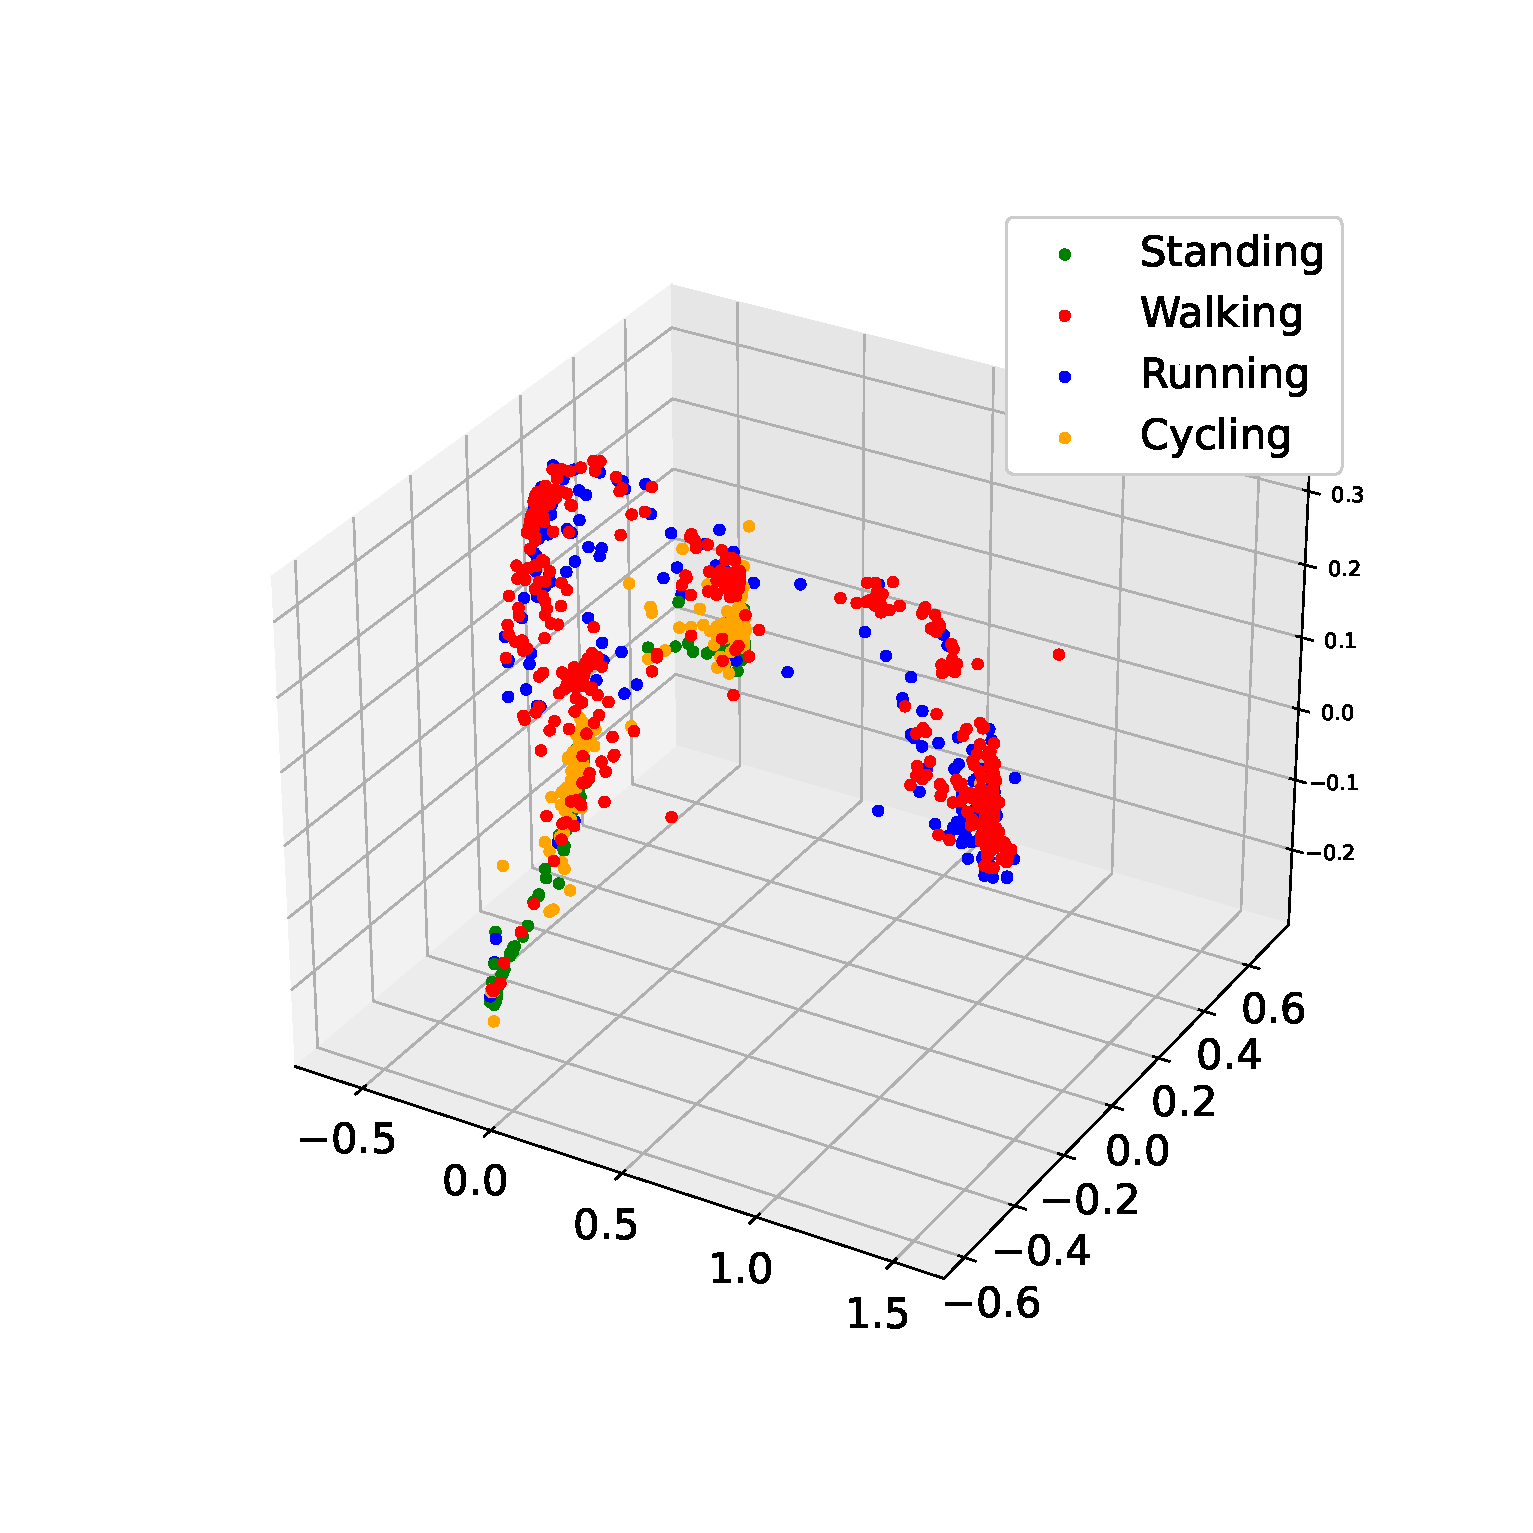
\includegraphics[width=0.5\textwidth]{Data_3D.eps}
            \caption{Распределения данных в 3D}
            \label{fig: 3D}
        \end{figure}

        \newpage

        Далее на рисунке \ref{fig: accuracy} приведено сравнение accuracy от количества главных компонент.

        \begin{figure}[H]
            \centering
            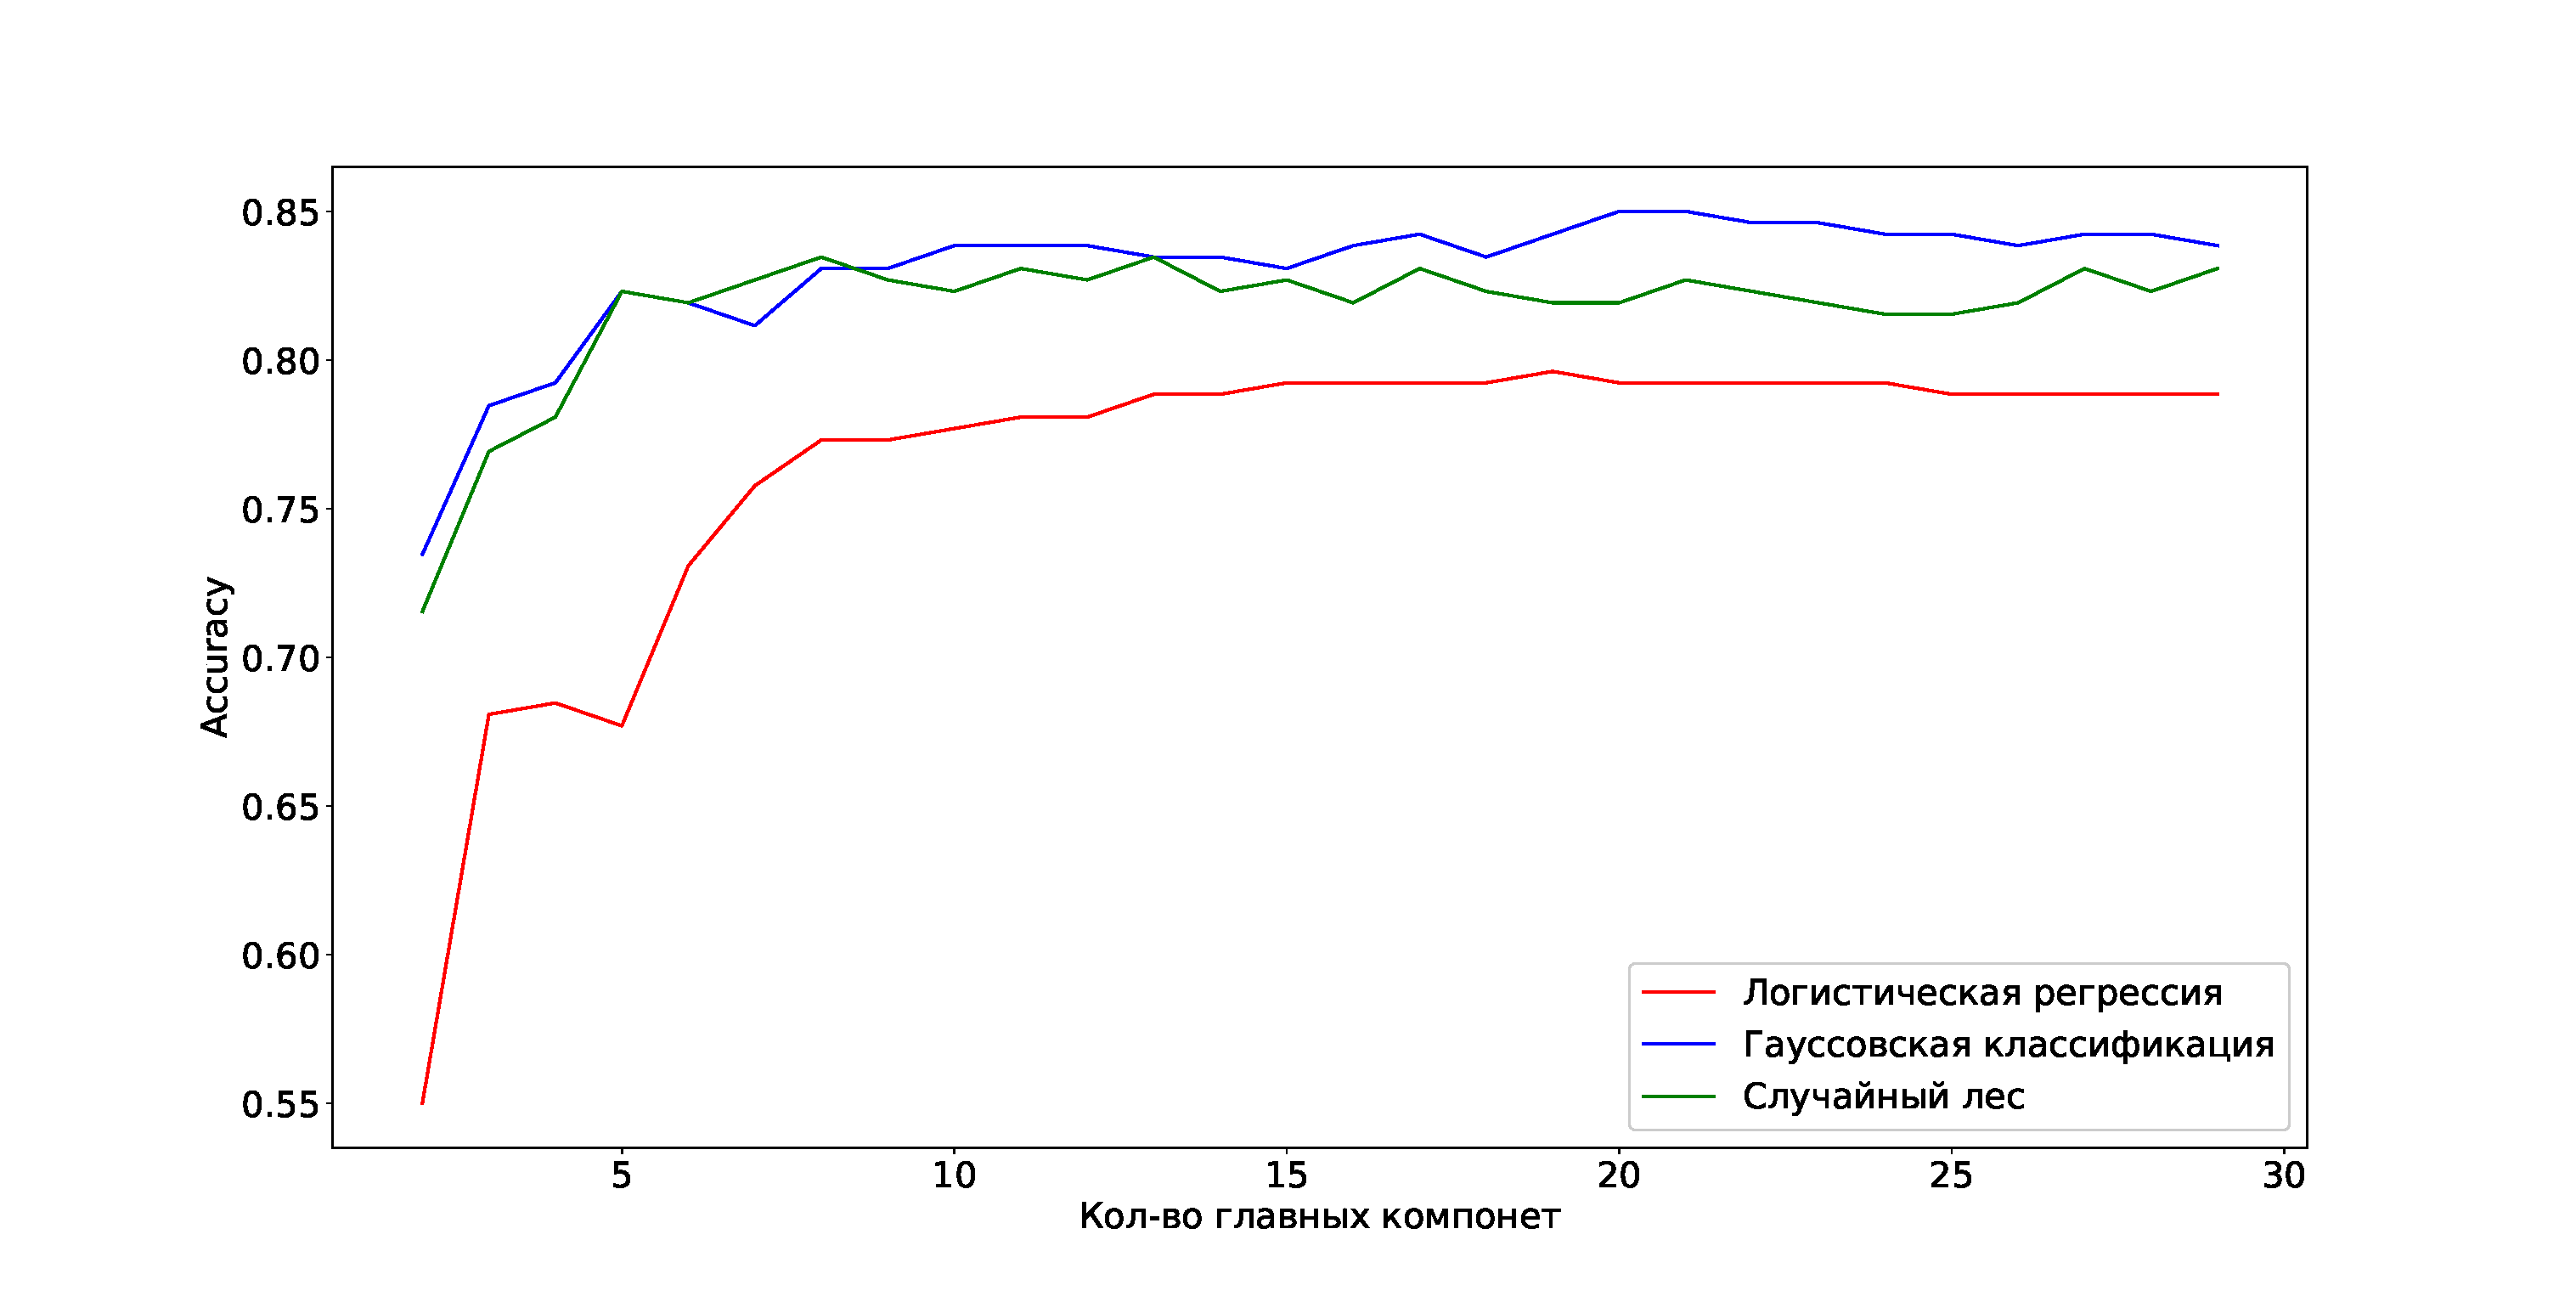
\includegraphics[width=\textwidth]{Accuracy.eps}
            \caption{Accuracy от количества главных компонент}
            \label{fig: accuracy}
        \end{figure}

        Наилучшее accuracy для различных классификаторов со стандартными параметрами:

        \begin{itemize}

            \item[$\bullet$] Логистическая регрессия: $79\%$

            \item[$\bullet$] Ядерный метод с гауссовским ядром: $85\%$

            \item[$\bullet$] Случайный лес: $83\%$

        \end{itemize}

\section{Заключение}

    Подтверждена гипотеза компактности: векторы параметров, соответствующие траекториям различных классов, оказываются разделимы в своём пространстве. Тем самым предложен метод решения задачи классификации динамических систем с помощью лагранжевой нейронной сети. Проведен вычислительный эксперимент на датасате PAMAP2, в которых проведено сравнение различных методов классификации.

\newpage

\bibliographystyle{plain}
\bibliography{Bogdanov2023LNN}

\end{document}
